%%%%%%%%%%%%%%%%%%%%%%%%%%%%%%%%%%%%%%%%%%%%%%%%%%%%%%%%%%%%%%%%%%%%%%%%%%%

\documentclass{standalone}

\usepackage{amsmath}
\usepackage{mathptmx}
\usepackage{pgfplots}
\usetikzlibrary{external}
\tikzexternalize{soup}
\pgfplotsset{compat=1.15}

%% IEEE uses Times Roman font, so we'll default to Times.
%% These three commands make up the entire times.sty package.
\renewcommand{\rmdefault}{ptm}
\renewcommand{\ttdefault}{pcr}
\normalfont\selectfont

\begin{document}

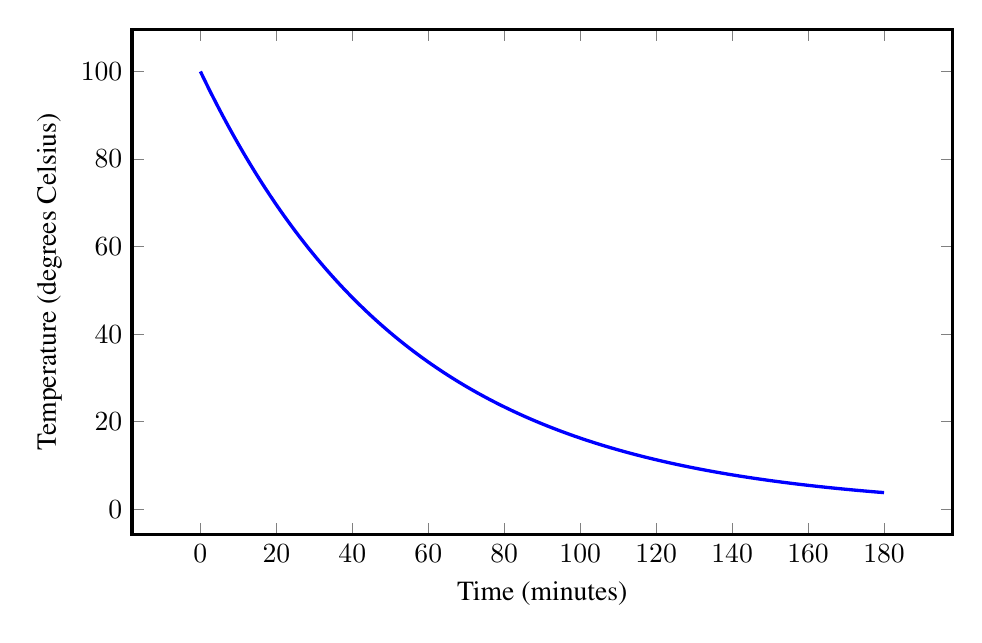
\begin{tikzpicture}
\tikzset{%%
  every mark/.append style={scale=1.0},%%
  scale=1.0%%
}
\pgfplotsset{%%
  every axis/.append style={font=\normalsize}%%
}
%%
\begin{axis}[%%
  axis line style=very thick,%%
  dotStyle/.style={very thick,blue,mark=none},%%
  enlargelimits=true,%%
  height=8cm,%%
  width=12cm,%%
  %% x axis
  xlabel={\normalsize Time~(minutes)},%%
  %% y axis
  ylabel={\normalsize Temperature~(degrees Celsius)},%%
  scaled y ticks=false,%%
  y tick label style=/pgf/number format/fixed%%
]
%%
%%
\addplot[dotStyle] coordinates {
  (0, 100.000000)
  (1, 98.200000)
  (2, 96.432400)
  (3, 94.696617)
  (4, 92.992078)
  (5, 91.318220)
  (6, 89.674492)
  (7, 88.060351)
  (8, 86.475265)
  (9, 84.918710)
  (10, 83.390174)
  (11, 81.889150)
  (12, 80.415146)
  (13, 78.967673)
  (14, 77.546255)
  (15, 76.150422)
  (16, 74.779715)
  (17, 73.433680)
  (18, 72.111874)
  (19, 70.813860)
  (20, 69.539211)
  (21, 68.287505)
  (22, 67.058330)
  (23, 65.851280)
  (24, 64.665957)
  (25, 63.501969)
  (26, 62.358934)
  (27, 61.236473)
  (28, 60.134217)
  (29, 59.051801)
  (30, 57.988868)
  (31, 56.945069)
  (32, 55.920057)
  (33, 54.913496)
  (34, 53.925054)
  (35, 52.954403)
  (36, 52.001223)
  (37, 51.065201)
  (38, 50.146028)
  (39, 49.243399)
  (40, 48.357018)
  (41, 47.486592)
  (42, 46.631833)
  (43, 45.792460)
  (44, 44.968196)
  (45, 44.158768)
  (46, 43.363910)
  (47, 42.583360)
  (48, 41.816860)
  (49, 41.064156)
  (50, 40.325001)
  (51, 39.599151)
  (52, 38.886366)
  (53, 38.186412)
  (54, 37.499056)
  (55, 36.824073)
  (56, 36.161240)
  (57, 35.510338)
  (58, 34.871152)
  (59, 34.243471)
  (60, 33.627089)
  (61, 33.021801)
  (62, 32.427409)
  (63, 31.843715)
  (64, 31.270528)
  (65, 30.707659)
  (66, 30.154921)
  (67, 29.612132)
  (68, 29.079114)
  (69, 28.555690)
  (70, 28.041687)
  (71, 27.536937)
  (72, 27.041272)
  (73, 26.554529)
  (74, 26.076548)
  (75, 25.607170)
  (76, 25.146241)
  (77, 24.693609)
  (78, 24.249124)
  (79, 23.812639)
  (80, 23.384012)
  (81, 22.963100)
  (82, 22.549764)
  (83, 22.143868)
  (84, 21.745278)
  (85, 21.353863)
  (86, 20.969494)
  (87, 20.592043)
  (88, 20.221386)
  (89, 19.857401)
  (90, 19.499968)
  (91, 19.148969)
  (92, 18.804287)
  (93, 18.465810)
  (94, 18.133425)
  (95, 17.807024)
  (96, 17.486497)
  (97, 17.171740)
  (98, 16.862649)
  (99, 16.559121)
  (100, 16.261057)
  (101, 15.968358)
  (102, 15.680928)
  (103, 15.398671)
  (104, 15.121495)
  (105, 14.849308)
  (106, 14.582021)
  (107, 14.319544)
  (108, 14.061792)
  (109, 13.808680)
  (110, 13.560124)
  (111, 13.316042)
  (112, 13.076353)
  (113, 12.840979)
  (114, 12.609841)
  (115, 12.382864)
  (116, 12.159972)
  (117, 11.941093)
  (118, 11.726153)
  (119, 11.515082)
  (120, 11.307811)
  (121, 11.104270)
  (122, 10.904393)
  (123, 10.708114)
  (124, 10.515368)
  (125, 10.326092)
  (126, 10.140222)
  (127, 9.957698)
  (128, 9.778459)
  (129, 9.602447)
  (130, 9.429603)
  (131, 9.259870)
  (132, 9.093193)
  (133, 8.929515)
  (134, 8.768784)
  (135, 8.610946)
  (136, 8.455949)
  (137, 8.303742)
  (138, 8.154274)
  (139, 8.007497)
  (140, 7.863362)
  (141, 7.721822)
  (142, 7.582829)
  (143, 7.446338)
  (144, 7.312304)
  (145, 7.180683)
  (146, 7.051430)
  (147, 6.924505)
  (148, 6.799863)
  (149, 6.677466)
  (150, 6.557272)
  (151, 6.439241)
  (152, 6.323334)
  (153, 6.209514)
  (154, 6.097743)
  (155, 5.987984)
  (156, 5.880200)
  (157, 5.774356)
  (158, 5.670418)
  (159, 5.568350)
  (160, 5.468120)
  (161, 5.369694)
  (162, 5.273039)
  (163, 5.178125)
  (164, 5.084919)
  (165, 4.993390)
  (166, 4.903509)
  (167, 4.815246)
  (168, 4.728571)
  (169, 4.643457)
  (170, 4.559875)
  (171, 4.477797)
  (172, 4.397197)
  (173, 4.318047)
  (174, 4.240322)
  (175, 4.163997)
  (176, 4.089045)
  (177, 4.015442)
  (178, 3.943164)
  (179, 3.872187)
  (180, 3.802488)
};
\end{axis}
\end{tikzpicture}

\end{document}
